\documentclass[11pt,letterpaper]{article}
\usepackage[margin=1in]{geometry}
\usepackage[T1]{fontenc}
\usepackage{newtxtext,newtxmath}
\usepackage{graphicx,booktabs,xcolor,amsmath,microtype,enumitem,caption,array}
\usepackage[hidelinks]{hyperref}
\captionsetup{font=small,labelfont=bf}
\setlist{itemsep=2pt,topsep=4pt,leftmargin=1.4em}
\setlength{\parskip}{4pt}
\definecolor{cgray}{HTML}{52514e}
\definecolor{cpanel}{HTML}{f0efec}
\newcommand{\code}[1]{\texttt{\small #1}}
\newcommand{\lw}{\lambda_{\text{w}}}

\title{\Large\bfseries TableNet: Where the Wheel Gap Comes From\\[2pt]\large What the 14--15 October runs showed,
and how each conclusion was reached}
\author{Research note. Companion to \emph{TableNet: One Network for Picks and Wheels} (\code{architecture.tex})}
\date{\small 15 October 2026}

\begin{document}
\maketitle

\noindent\colorbox{cpanel}{\parbox{\dimexpr\linewidth-2\fboxsep}{\small
\textbf{In short.} After step~2, TableNet (the all-sets PickNet plus a wheel head, trained together) trailed the
per-set WheelNets by 0.5\% in wheel log loss. Four findings explain the gap:
\begin{enumerate}[leftmargin=1.6em,itemsep=1pt,topsep=2pt]
\item \textbf{The wheel task was under-trained.} Raising the wheel weight from 0.3 to 3, or training a second
pass, takes TableNet past the per-set WheelNets on average ($-$0.22\%).
\item \textbf{The wheel loss does not help picks.} The pick gains seen in step~2 come from fine-tuning itself.
Above a wheel weight of 1, picks start to pay a small price.
\item \textbf{The two tasks disagree in one place: the history encoder.} This is the part of PickNet that
summarizes the draft so far. Elsewhere their gradients are close to orthogonal.
\item \textbf{The history encoder is also where the extra wheel accuracy comes from.} Keeping the wheel loss out
of it protects picks, but loses all the gain.
\end{enumerate}
\textbf{Conclusion:} the wheel task needs the history summarized differently from the pick task, so it should get
history capacity of its own. Two runs testing exactly that are in progress (Section~\ref{sec:next}).}}

\section{The setup in one paragraph}

TableNet is PickNet's all-sets model (8.48M parameters, 19 Premier sets) with a 1.06M-parameter wheel head on top.
The wheel head predicts, for each card you pass at a wheel-eligible pick, whether it comes back eight picks later.
Training minimizes
\[ \mathcal L = \text{pick NLL} + 0.3\,\text{deck BCE} + \lw\,\text{wheel BCE}, \]
starting from step~1 (PickNet frozen, head trained). PickNet's learning rate is $5{\times}10^{-5}$ and the
head's $3{\times}10^{-4}$, for one pass over 285,000 drafts. Every number below is measured on all 19 sets'
chronological test drafts.
\begin{itemize}
\item \textbf{Wheel:} log loss, compared with each set's own WheelNet on exactly the same passed cards (16 sets
have one).
\item \textbf{Picks:} top-1 accuracy and NLL.
\item \textbf{The bar:} pick top-1 must stay within 0.1 points everywhere.
\end{itemize}

\section{How the conclusions were reached}\label{sec:method}

Three kinds of evidence were used, and each answers a different question.

\paragraph{1. Controlled runs: does changing X change the result?} Each run changes exactly one thing relative to
another run: the wheel weight, the number of passes, or which weights the wheel loss may touch. The training
drafts, their order, the seed, the schedule and the scorer stay the same. The scorer is checked at start-up
against PickNet's published MSH numbers, and it reproduced them exactly in every run.

The most important run is the \textbf{pick-only control}: the same fine-tune with $\lw=0$. Without it, pick
changes cannot be attributed to the wheel loss. Step~2 had raised FRA's pick top-1 by 0.29 points and HOB's by
0.21, which looked like the wheel task helping picks. The control shows the same gains with no wheel loss at all.
They came from the first full training on those two sets' drafts.

\paragraph{2. Consistency across 19 sets: is a small effect real?} Each configuration was run once, with one
seed, so there is no run-to-run spread to compare against. Instead, the 19 sets serve as 19 separate test beds.
An effect of $-$0.01 points in pick top-1 would be noise on one set. When it has the same sign on 17 of 19 sets,
and NLL moves the same way on 18 of 19, it is a real (if tiny) effect. Every comparison below reports this count.

\paragraph{3. Gradient geometry: where in the network do the tasks disagree?} For a trained checkpoint, we take the
gradient of each loss separately with respect to PickNet's weights, and compare their directions within each part
of the network (card table, history inputs, each history layer, each decoder block) using the cosine.
\begin{itemize}
\item \textbf{Cosine $>0$:} the two tasks want the same change.
\item \textbf{Cosine $\approx0$:} they don't interact.
\item \textbf{Cosine $<0$:} they pull against each other.
\end{itemize}
Two versions are computed over 1000 training batches (\code{scripts/grad\_cosine.py}):
\begin{itemize}
\item \textbf{Per-batch cosine.} This is about 0 everywhere ($\pm0.04$). A single batch of 32 drafts is dominated
by noise, so per-batch cosines say little.
\item \textbf{Cosine of the batch-averaged gradients.} Averaging cancels the noise and leaves the direction each
loss pushes on average. This is the informative one.
\end{itemize}
One caveat matters for reading it. At a fully trained checkpoint, the weighted gradients sum to about zero:
$\nabla\text{pick} + 0.3\,\nabla\text{deck} + \lw\nabla\text{wheel} \approx 0$. So some anti-alignment is
built in. The script therefore also reports the size of the averaged gradient. It is about 4\% of the per-batch
size for both losses, which confirms that the checkpoints are near that balance point. The cosine is still
informative about \emph{where} the tasks have to compromise. And the step-1 checkpoint, whose PickNet had never
seen the wheel loss, shows the same pattern.

\paragraph{4. Intervention: is that part of the network actually responsible?} The gradient analysis says where the
tasks disagree. It doesn't say what happens if the disagreement is removed. To test that directly, we reran
$\lw=3$ with the wheel loss's gradient blocked from the history encoder and its input embeddings (3.44M of
PickNet's 8.48M weights; option \code{wheel\_block=hist}). Those weights then train on picks and decks only.
Everything else is unchanged.

\section{Findings}

\begin{table}[h]
\centering\small
\begin{tabular}{lcccc}
\toprule
& wheel log loss & \multicolumn{2}{c}{pick top-1 vs.\ control (pt)} & pick NLL \\
\cmidrule(lr){3-4}
run & vs.\ WheelNet (mean) & mean & worst set & vs.\ control \\
\midrule
step 1: frozen PickNet & +0.92\% & --- & --- & --- \\
pick-only control, $\lw=0$ & (not trained) & 0 & 0 & 0 \\
$\lw=0.3$ (step 2) & +0.53\% & $-$0.001 & $-$0.02 & 0.0000 \\
$\lw=1$ & +0.19\% & $-$0.010 & $-$0.03 & +0.0002 \\
$\lw=1$, second pass & $-$0.10\% & $-$0.013 & $-$0.08 (MOM) & +0.0004 \\
$\lw=3$ & \textbf{$-$0.22\%} & $-$0.034 & $-$0.09 (HOB) & +0.0012 \\
$\lw=3$, history encoder blocked & +0.22\% & $-$0.013 & $-$0.06 (HOB) & +0.0006 \\
\bottomrule
\end{tabular}
\caption{All runs, test drafts of all 19 sets. Wheel: mean over the 16 sets with a per-set WheelNet (negative
is better than WheelNet). Picks: change against the pick-only control.}
\label{tab:runs}
\end{table}

\begin{figure}[h]
\centering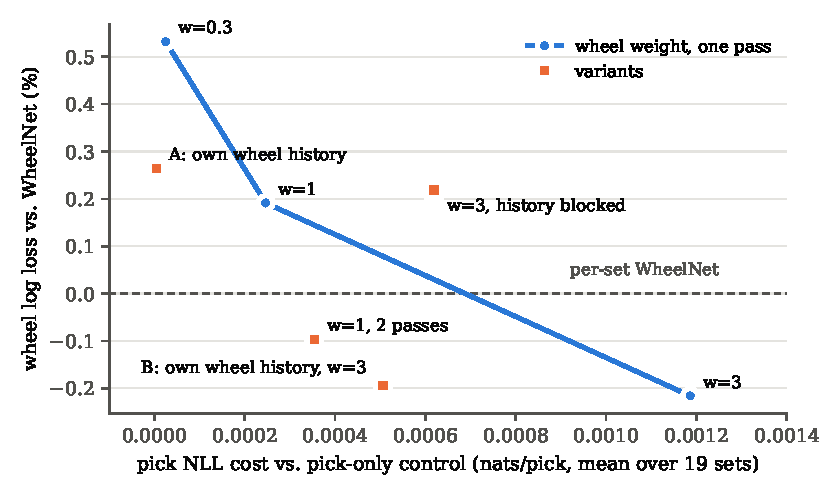
\includegraphics[width=0.82\linewidth]{figs/tradeoff.pdf}
\caption{The pick/wheel trade-off; down and left is better. The blue line is the wheel-weight sweep (one pass
each). A second pass reaches nearly the same wheel accuracy as $\lw=3$ at a third of the pick cost. Blocking the
history encoder gives up the wheel gain. Run B (own wheel history encoder, PickNet's history blocked, $\lw=3$) matches
$\lw=3$'s wheels at a third of its pick cost.}
\label{fig:tradeoff}
\end{figure}

\subsection{The wheel task was under-trained}

\textit{Question.} Was the 0.5\% gap a limit of sharing the network, or just not enough training signal for the
wheel task?

\textit{How we found out.} We raised the wheel weight (0.3, then 1, then 3) and, separately, trained a second
pass at weight 1. The gradient analysis supplied the reason: the wheel loss's gradient on PickNet is about
\textbf{one-fifth} the size of the pick loss's (0.06 vs.\ 0.28). At $\lw=0.3$ it made up only about 6\% of each
update.

\textit{Result.} Each step helps on every one of the 19 sets.
\begin{itemize}
\item \textbf{$\lw=1$:} 0.30--0.41\% better than $\lw=0.3$.
\item \textbf{$\lw=3$:} another 0.33--0.53\% better. On average this is past the per-set WheelNets
($-$0.22\%, 11 of 16 sets at or past parity, all 16 within 1\%).
\item \textbf{Second pass at $\lw=1$:} 0.20--0.39\% better than one pass (mean 0.29\%).
\end{itemize}
Training longer is the cheaper route. It costs a third of $\lw=3$'s pick NLL for most of its wheel gain
(Figure~\ref{fig:tradeoff}). That comparison is slightly generous to the second pass, because there is no
two-pass pick-only control.

\subsection{The wheel loss does not help picks}

\textit{How we found out.} Compare the pick-only control with the runs that include the wheel loss.

\textit{Result.}
\begin{itemize}
\item \textbf{$\lw=0.3$:} identical to the control ($-$0.001 points).
\item \textbf{$\lw=1$:} $-$0.010 points, lower on 17 of 19 sets; NLL worse on 18 of 19.
\item \textbf{$\lw=3$:} $-$0.034 points, lower on 18 of 19. HOB ($-$0.09) and MOM ($-$0.08) come close to
the 0.1-point bar.
\end{itemize}
So there is no positive transfer from wheels to picks, and a cost that grows with the wheel weight. It is
negligible up to $\lw=1$.

\begin{figure}[t]
\centering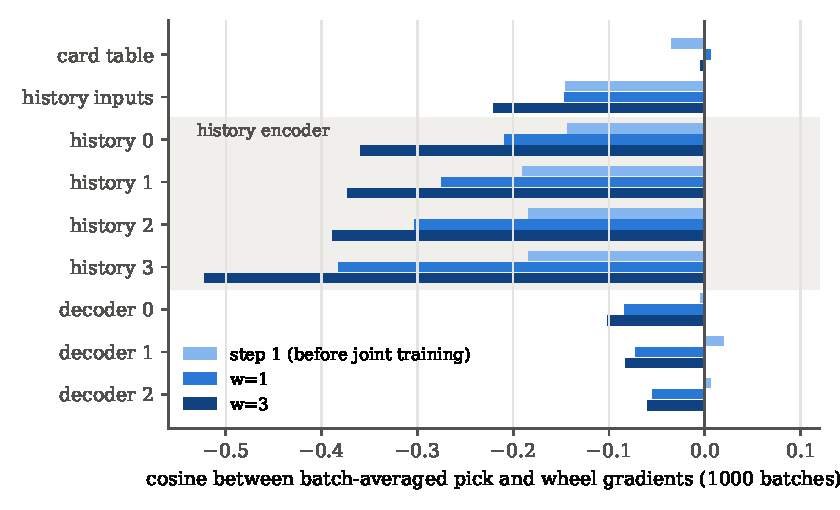
\includegraphics[width=0.82\linewidth]{figs/cosines.pdf}
\caption{Cosine between the batch-averaged pick and wheel gradients, per part of PickNet; negative means the tasks
pull against each other. The disagreement is in the history encoder (shaded) and grows with the wheel weight. The
card table and the pack decoder are close to neutral.}
\label{fig:cos}
\end{figure}

\subsection{The disagreement is in the history encoder}

\textit{How we found out.} We ran the gradient analysis of Section~\ref{sec:method} on three checkpoints: step~1,
$\lw=1$ and $\lw=3$ (Figure~\ref{fig:cos}).

\textit{Result.}
\begin{itemize}
\item \textbf{Card table:} pick and wheel are close to orthogonal ($\pm0.03$).
\item \textbf{Pack decoder:} near zero or slightly negative ($-0.01$ to $-0.10$).
\item \textbf{History encoder:} clearly opposed. Even at step~1, before the wheel loss had touched PickNet, the
cosine is $-0.14$ to $-0.19$. At $\lw=3$ it deepens to $-0.36$ to $-0.52$; the deepest layer is the most
negative.
\end{itemize}
The deck loss sides with picks: pick vs.\ deck is $+0.05$ to $+0.31$, and deck vs.\ wheel is negative in the
same layers. This fits what the history encoder is for. It summarizes \emph{my} picks and plan, which is what
picks and deck-building need. Predicting wheels needs a summary of what the \emph{other} seats are taking.

\subsection{The history encoder is also where the wheel gain comes from}

\textit{How we found out.} The intervention described in Section~\ref{sec:method}: $\lw=3$ with the wheel gradient
blocked from the history encoder.

\textit{Result.}
\begin{itemize}
\item \textbf{Wheels:} the blocked run is 0.37--0.56\% worse than $\lw=3$ on \emph{every} set, and level with
$\lw=1$ on average. All of the gain from raising the weight disappears.
\item \textbf{Picks:} about two-thirds of the cost comes back. Top-1 is $-$0.013 against the control (vs.\
$-$0.034), and NLL is +0.0006 (vs.\ +0.0012). The remainder comes from the card table and decoder, which the
wheel loss could still change.
\end{itemize}

\textit{What it means.} The wheel loss can only improve wheels further by reshaping the history summary, and
that is exactly what costs picks. The usual fixes for conflicting tasks either block a component or project out
conflicting gradient directions (PCGrad). Here they would protect picks only by giving up the wheel gain. The
better fix is to give the wheel task \emph{its own} history capacity, so neither task has to compromise.

\section{Limits of these conclusions}

\begin{itemize}
\item \textbf{One seed per configuration.} Effects are judged by their consistency across 19 sets, not by repeated
runs. The wheel effects are large relative to that check (same sign on 19 of 19 sets in every comparison). The
pick effects at $\lw\le1$ are real but tiny.
\item \textbf{The per-set WheelNet is a weak baseline.} Most per-set WheelNets lack the draft-date context of the
newer ones. On MSH, the best TableNet run (0.4224) is still behind \code{wheelnet\_time} (0.4218) and the
multi-set WheelNet (0.4188). Beating those is the real bar.
\item \textbf{The second-pass run has no matching two-pass control}, so its pick numbers are slightly flattering.
\item \textbf{The four hardest sets are the same in every run} (BLB, ECL, HOB, SOS). Nothing tried so far
addresses whatever makes them hard.
\item \textbf{One run was paused at the operating-system level for 75 minutes} (the pick-only control,
probably under memory pressure). It resumed from the same state, so its results are unaffected; only its logged
timings are off.
\end{itemize}

\section{Follow-up: a history encoder for the wheel head}\label{sec:next}

\code{train\_tablenet\_joint.py whist\_layers=2} adds a separate 2-layer causal history encoder (1.93M
parameters) used only by the wheel head.
\begin{itemize}
\item \textbf{Inputs:} the same as PickNet's history, read through PickNet's card table.
\item \textbf{Output:} added to the wheel head's tokens at each wheel slot, through a projection initialized to
zero. Training therefore starts exactly at the step-1 head (MSH wheel 0.4267, reproduced).
\item \textbf{Leakage check:} at start-up, a check confirms that its state at pick $t$ ignores every later pick.
\end{itemize}
Two runs (\code{results/tablenet/run\_whist.sh}, \code{run\_whist\_b.sh}):
\begin{enumerate}[label=\Alph*.]
\item \textbf{Wheel loss kept out of PickNet entirely} (\code{wheel\_block=all}, $\lw=1$). Picks then train exactly
as in the control, so any wheel improvement is pure gain. \emph{Success:} wheel log loss at or below the $\lw=1$
run (+0.19\%) with picks equal to the control.
\item \textbf{Wheel loss kept out of PickNet's history encoder only} (\code{wheel\_block=hist}, $\lw=3$). The wheel
task can still shape the card table and decoder, where the tasks don't conflict. \emph{Success:} wheel log loss
at or below $\lw=3$ ($-$0.22\%) at the blocked run's pick cost or less.
\end{enumerate}

\paragraph{Run A result.} Picks are identical to the control, as designed: top-1 $+0.002$ points, NLL
$+0.000005$. Wheel log loss is $+0.26\%$ against the per-set WheelNet, about the $\lw=1$ level ($+0.06\%$ from it,
better on 6 of 19 sets) and 0.31--0.61\% behind $\lw=3$ on every set.
\begin{itemize}
\item \textbf{The good news:} a wheel-only history encoder buys the $\lw=1$ wheel accuracy with no pick cost.
\item \textbf{The limit:} it adds nothing beyond that. The extra gain at $\lw=3$ came from reshaping PickNet's
shared parts, which a separate history summary does not reproduce. So the wheel head was not short of history
information.
\item \textbf{Still open:} whether PickNet's features help the wheel task at all. On MSH, the multi-set WheelNet,
which uses no PickNet, is still the best wheel model (0.4188, vs.\ 0.4224 for TableNet's best). The next test is an
ablation ladder that removes PickNet's history, then its representations, then its card table from the wheel head.
\end{itemize}

\paragraph{Run B result: the best trade-off so far.}
\begin{itemize}
\item \textbf{Wheels:} the same accuracy as $\lw=3$ ($-0.19\%$ against the per-set WheelNet; $+0.01\%$ from
$\lw=3$, better on 9 of 19 sets). 11 of 16 sets are at or past parity.
\item \textbf{Picks:} a third of $\lw=3$'s pick cost. Top-1 is $-0.010$ points against the control (worst set HOB,
$-0.05$), and NLL is $+0.0005$ (vs.\ $+0.0012$).
\item \textbf{Pick AUC}, the first run to report it: 0.953 pooled and 0.910 within-pack, averaged over the 19 sets.
On MSH, 0.9505 vs.\ 0.9506 for the starting PickNet.
\end{itemize}
Set side by side with the blocked run (Figure~\ref{fig:tradeoff}), B shows that the wheel task needs two things:
its own summary of the draft, and the freedom to adjust the shared card table and pack decoder, where the tasks
don't conflict. Neither alone is enough. The remaining pick cost comes from those shared parts.

B still does not beat the strongest pure WheelNet. On MSH it scores 0.4227 against the multi-set WheelNet's
0.4188. A multi-set WheelNet for all 19 sets (one model per pack size, scored on exactly TableNet's test examples)
is written and tested (\code{scripts/train\_wheelnet\_allsets.py}), and will show whether that gap holds on every
set.

\section{Reproducing}

\begin{itemize}
\item \textbf{Runs:} \code{scripts/train\_tablenet\_joint.py} with \code{wheel\_w}, \code{resume},
\code{wheel\_block} and \code{whist\_layers}. Queue scripts are \code{results/tablenet/run\_*.sh}.
\item \textbf{Results:} \code{results/tablenet/tablenet\_joint\_*.json} and \code{.log}.
\item \textbf{Gradient analysis:} \code{scripts/grad\_cosine.py} writes \code{results/tablenet/grad\_cosine*.json}.
\item \textbf{Figures:} \code{paper/combined/figs/make\_overnight\_figs.py}, which reads those JSON files.
\item \textbf{Running notes and full per-set tables:} \code{paper/combined/gap-diagnosis.md}.
\end{itemize}

\end{document}
